%%%%%%%%%%%%%%%%%%%%%%%%%%%%%%%%%%%%%%%%%
% Dreuw & Deselaer's Poster
% LaTeX Template
% Version 1.0 (11/04/13)
%
% Created by:
% Philippe Dreuw and Thomas Deselaers
% http://www-i6.informatik.rwth-aachen.de/~dreuw/latexbeamerposter.php
%
% This template has been downloaded from:
% http://www.LaTeXTemplates.com
%
% License:
% CC BY-NC-SA 3.0 (http://creativecommons.org/licenses/by-nc-sa/3.0/)
%
%%%%%%%%%%%%%%%%%%%%%%%%%%%%%%%%%%%%%%%%%

%----------------------------------------------------------------------------------------
%	PACKAGES AND OTHER DOCUMENT CONFIGURATIONS
%----------------------------------------------------------------------------------------

\documentclass[final,hyperref={pdfpagelabels=false}]{beamer}

\usepackage[orientation=portrait,size=a1]{beamerposter} % Use the beamerposter package for laying out the poster with a portrait orientation and an a0 paper size

\usetheme{I6pd2} % Use the I6pd2 theme supplied with this template

\usepackage[english]{babel} % English language/hyphenation

\usepackage{amsmath,amsthm,amssymb,latexsym} % For including math equations, theorems, symbols, etc

%\usepackage{times}\usefonttheme{professionalfonts}  % Uncomment to use Times as the main font
%\usefonttheme[onlymath]{serif} % Uncomment to use a Serif font within math environments

\boldmath % Use bold for everything within the math environment

\usepackage{booktabs} % Top and bottom rules for tables

\graphicspath{{figures/}} % Location of the graphics files

\usepackage{subfigure}
\usepackage{xeCJK}
	\setCJKmainfont{cwTeX Q HeiZH}

\usecaptiontemplate{\small\structure{\insertcaptionname~\insertcaptionnumber: }\insertcaption} % A fix for figure numbering

%----------------------------------------------------------------------------------------
%	TITLE SECTION 
%----------------------------------------------------------------------------------------

\title{\huge So, Where Are the Ads?} % Poster title

\author{B02705008 江昱熹、B02902056 江韋霖、B02902034 邱筱晴、B02705019陳姿穎} % Author(s)

\institute{Computer Science and Information Engineering, National Taiwan University } % Institution(s)

%----------------------------------------------------------------------------------------
%	FOOTER TEXT
%----------------------------------------------------------------------------------------

\newcommand{\leftfoot}{} % Left footer text

\newcommand{\rightfoot}{} % Right footer text

%----------------------------------------------------------------------------------------

\begin{document}

\addtobeamertemplate{block end}{}{\vspace*{2ex}} % White space under blocks

\begin{frame}[t] % The whole poster is enclosed in one beamer frame

\begin{columns}[t] % The whole poster consists of two major columns, each of which can be subdivided further with another \begin{columns} block - the [t] argument aligns each column's content to the top

\begin{column}{.02\textwidth}\end{column} % Empty spacer column

\begin{column}{.465\textwidth} % The first column

%----------------------------------------------------------------------------------------
%	OBJECTIVES
%----------------------------------------------------------------------------------------

%\begin{block}{Objectives}

%\begin{enumerate}
%\item Donec fringilla, velit id lobortis commodo, eros dui %consectetur mi, ut interdum lorem dui sed mauris.
%\item Nulla ac nulla rhoncus est bibendum ullamcorper:
%\item Quisque vestibulum, nisl sit amet gravida ultricies dis %parturient montes, nascetur ridiculus musobortis commodo, eros %dui consectetur mi.
%\end{enumerate}

%\end{block}

%----------------------------------------------------------------------------------------
%	INTRODUCTION
%----------------------------------------------------------------------------------------
            
\begin{block}{Introduction}

\par Instagram is an online mobile photo-sharing, video-sharing and social networking service, which rapidly gained popularity, with over 300 million as of December 2014. One of the features in Instagram is that users can add hashtags on their photos. Using specific tags can help users connect with other like-minded people on Instagram. For example, when searching \#cat on Instagram, users can explore many special and cute photos related to cats. 

\quad Therefore, we wonder whether the Chinese hashtags on Instagram are also fancy. We searched hashtags such as \#台灣,  expecting to get some beautiful scene in Taiwan. Unfortunately, there are so many spamming and advertising posts! We think that will be a very bad experience for users.Thus, we aim to imporve the quility of Chinese hashtags and try to classify the spam posts by using machine learning techniques.

\begin{figure}
\centering
\subfigure[An example of normal post in \#台灣]{
	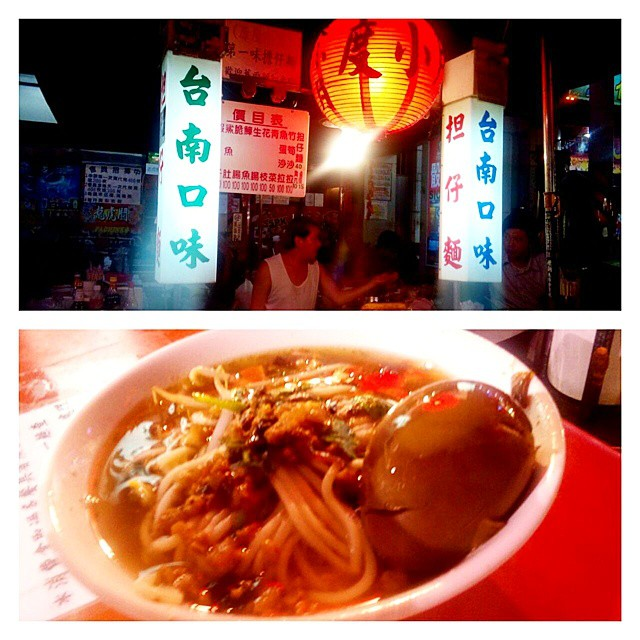
\includegraphics[width=0.3\linewidth]{normpost.jpg}
}
\hspace{1em}
\subfigure[An example of spam post in \#台灣]{
	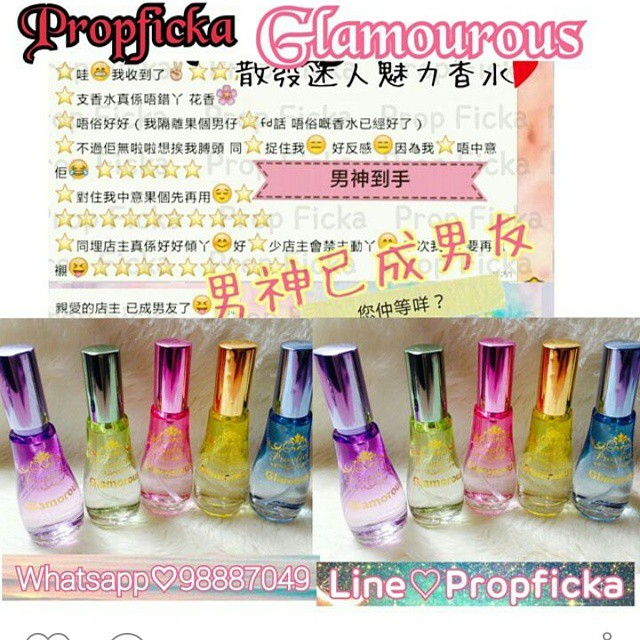
\includegraphics[width=0.3\linewidth]{spampost.jpg}
}
\end{figure}


\end{block}

%----------------------------------------------------------------------------------------
%	MATERIALS
%----------------------------------------------------------------------------------------

\begin{block}{Workflow}

%\begin{columns} % Subdivide the first main column
%\begin{column}{.54\textwidth} % The first subdivided column %within the first main column
%\begin{itemize}
%\item Vestibulum nisl, quis euismod velit eros in ligula.
%\begin{itemize}
%\item Cras rhoncus quam et augue convallis in elementum urna %tincidunt.
%\end{itemize}
%\item Proin ut vestibulum augue.
%\begin{itemize}
%\item Donec dapibus sagittis neque eu ultrices.
%\end{itemize}
%\end{itemize}
%\end{column}

%\begin{column}{.43\textwidth} % The second subdivided column within the first main column

First, we collect many posts with different hashtags from Instagram. Then classify whether a post is spamming manually by a tool we write. After classifying posts, we divide the data into two parts of same size, which correspond to training data and testing data. In training data, we try hard to observe some features in spam posts and come up with some measurable properties, which we will discuss the result detailly in Section Model. In Section Method, we will compare the performance of some popular machine learning techniques with different features selection. Finally, our ultimate goal is to provide a useful web application for users. 

\centering
\begin{figure}

\includegraphics[scale=1]{workflow.png}
\caption{Workflow of the project.}
\end{figure}
%\end{column}
%\end{columns} % End of the subdivision


\end{block}

%----------------------------------------------------------------------------------------
%	OBSERVATION AND FEATURE EXTRACTION
%----------------------------------------------------------------------------------------

\begin{block}{Observation and Feature Extraction}



%\begin{description}
\begin{tabular}{ll}
Digits & Advertisers often need to provide the contact way, such as phone numbers. \\
Hashtags & Advertisers usually use many tags to let the post easily appear in search results. \\
Social media & Advertisers sometimes will provide social accounts such as Line, whatsapp, Facebook, etc. \\
Keywords & We try to find the keywords which advertisers often use in posts by some analysis.

\end{tabular}

\end{block}


%----------------------------------------------------------------------------------------
%	METHODS
%----------------------------------------------------------------------------------------

\begin{block}{Feature Sets Details}


\begin{itemize}
\item Feature Set 1
	\begin{itemize}
		\item Based on the observation above, we come up with some simple features at first, which includes \texttt{tag-amount}, \texttt{longest-digits}, \texttt{social-media}, \texttt{keyword-count}, ..., totally 11 features. In particular \texttt{keyword-count}, we only consider about ten words produced by us. Notice that we consider not only the content in posts, but also the info page of authors. We think that makes sense since advertisers usually put the contact info to author description. 
	\end{itemize}
\item Feature Set 2
	\begin{itemize}
		\item However, it is not enough to become a general model by using only ten keywords. Therefore, we take some analysis on the training data by a Chinese text segmentation tool called \texttt{jieba}. By using the tool, we count frequency of each word and select the ones occur more than 50 times, and then pick the words as the features, representing how many times the words appear in contents. The method actually called uni-gram in Language Model. Similarly, we also take Chinese character into consideration, and finally the number of features will up to 1000.
	\end{itemize}
\end{itemize}
\end{block}



%----------------------------------------------------------------------------------------
%	Data Description
%----------------------------------------------------------------------------------------

\begin{block}{Data Description}

We collect total 1920 posts, in which a hashtag consist of 60 posts, and randomly split the hashtags into two parts with same posts size 960. Note that we do not random by posts, since we want to examine whether our model would still perform well on different hashtags.

\begin{table}[h]
\centering
\caption{Data Description}
\label{data-table}
\begin{tabular}{lll}
\multicolumn{1}{l|}{Hashtags (top - training data, bottom - testing data)}                                                                                 & \multicolumn{1}{l|}{spam} & not spam \\ \hline
\multicolumn{1}{l|}{\begin{tabular}[c]{@{}l@{}}文青、日本、母親節、吃飯、龍貓、早安、蔬菜、都敏俊\\ 蛋黃哥、夏天、五月天、運動、髮型、馬卡龍、台灣、正妹\end{tabular}} & \multicolumn{1}{l|}{417}  & 543      \\ \hline
\multicolumn{1}{l|}{\begin{tabular}[c]{@{}l@{}}天氣、哭、可愛、人生、廢話、香港、生日快樂、羊駝\\ 迪士尼、夜景、閃光、美食、腳踏車、海邊、北海道、貓咪\end{tabular}}  & \multicolumn{1}{l|}{726}  & 234      \\
                                                                                                                    &                           &          \\
                                                                                                                    &                           &          \\
                                                                                                                    &                           &         
\end{tabular}
\end{table}
\end{block}

%----------------------------------------------------------------------------------------
%	MATHEMATICAL SECTION
%----------------------------------------------------------------------------------------

%\begin{block}{Mathematical Section}

%\begin{itemize}
%\item Maecenas Ultricies Feugiat Velit Non Mattis.
%\begin{itemize}
%\item Duis ante erat, bibendum nec tempus nec, interdum quis est. Nulla at mollis %tortor. Phasellus quis leo dolor, aliquam laoreet orci $X$ Donec dapibus sagittis %neque eu nec, interdum quis est. $Y_n, n=1,\cdots,N$ ndum nec tempus nec, interd
%\begin{align*}
%X \rightarrow r(X) & = \arg \max_{c} \Big\{ \max_n \big\{ \sum_{x_i \in X} %\delta(x_i,Y_{n,c})\big\} \Big\} 
%\end{align*}
%\item Cras faucibus scelerisque cursus. Proin ut vestibulum augue. $\delta(x_i,Y_{n,c})$
%\end{itemize}
%\item Fusce tempus arcu id ligula varius dictum. Donec ut nisl dui, ac consectetur elit. In nec enim porta augue venenatis sollicitudin. Phasellus quis nunc neque. Suspendisse mauris diam, suscipit non gravida in, placerat id enim. Ut nec ipsum in lectus ultrices sagittis.
%\end{itemize}

%\end{block}

%----------------------------------------------------------------------------------------

\end{column} % End of the first column

\begin{column}{.03\textwidth}\end{column} % Empty spacer column
 
\begin{column}{.465\textwidth} % The second column

%----------------------------------------------------------------------------------------
%	METHOD
%----------------------------------------------------------------------------------------

\begin{block}{METHOD}

\begin{columns}

\begin{column}{.5\textwidth}
\begin{itemize}

\item \texttt{Decision Tree} \\
	%\begin{itemize}
	%	\item 
		Decision tree is a classification algorithm that performs a recursive binary partitioning of the feature space. The tree predicts the same label for each leaf partition. Each partition is chosen by selecting the best split from a set of possible splits, in order to maximize the information gain at a tree node. Here we directly use the implementation in the library scikit-learn.
	%\end{itemize}
\item \texttt{Random Forests}
	
\item Linear Support Vector Machines

\item Kernel Support Vector Machines
\end{itemize}

\end{column}

\begin{column}{.4\textwidth}

\begin{figure}
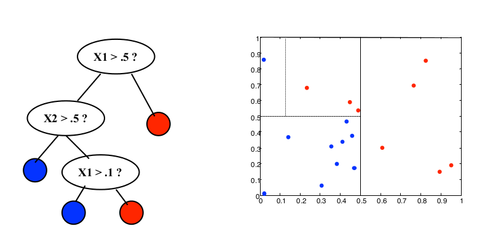
\includegraphics[width=1\linewidth]{decision_tree.png}
\caption{Decision tree}
\end{figure}

\end{column}

\end{columns}





%\begin{table}
%\begin{tabular}{l l l}
%\toprule
%\textbf{Treatments} & \textbf{Response 1} & \textbf{Response 2}\\
%\midrule
%Treatment 1 & 0.0003262 & 0.562 \\
%Treatment 2 & 0.0015681 & 0.910 \\
%Treatment 3 & 0.0009271 & 0.296 \\
%\bottomrule
%\end{tabular}
%\caption{Table caption}
%\end{table}

%\begin{itemize}
%\item Sollicitudin Vel Orci
%\item Maecenas Ultricies Feugiat Velit Non Mattis.
%\end{itemize}

%\begin{table}
%\begin{tabular}{l l l}
%\toprule
%\textbf{Treatments} & \textbf{Response 1} & \textbf{Response 2}\\
%\midrule
%Treatment 1 & 0.0003262 & 0.562 \\
%Treatment 2 & 0.0015681 & 0.910 \\
%Treatment 3 & 0.0009271 & 0.296 \\
%\bottomrule
%\end{tabular}
%\caption{Table caption}
%\end{table}
     
\end{block}

%------------------------------------------------

\begin{block}{Results: Figure}

\begin{figure}

\includegraphics[width=0.8\linewidth]{placeholder.jpg}
\caption{Figure caption}
\end{figure}

\end{block}

%----------------------------------------------------------------------------------------
%	CONCLUSION
%----------------------------------------------------------------------------------------

\begin{block}{Conclusion}

\begin{itemize}
\item Opet volutpat ligula. Duis semper lorem eget dui dignissim porttitor. Nulla facilisi. In ullamcorper lorem quis dolor iaculis nec egestas enim ultricies. Cras ut mauris elit, ut lacinia dui. Proin in ante et libero hendrerit iaculis.
\item Nulla eu erat a urna laoreet auctor id a turpis. Nam mollis tristique neque eu luctus. Suspendisse rutrum congue nisi sed convallis. 
\item Aenean id neque dolor.
\item Opet volutpat ligula. Duis semper lorem eget dui dignissim porttitor. Nulla facilisi. In ullamcorper lorem quis dolor iaculis nec egestas enim ultricies. Cras ut mauris elit, ut lacinia dui. Proin in ante et libero hendrerit iaculis.
\end{itemize}

\end{block}

%----------------------------------------------------------------------------------------
%	REFERENCES
%----------------------------------------------------------------------------------------

\begin{block}{References}
        
\nocite{*} % Insert publications even if they are not cited in the poster
\small{\bibliographystyle{unsrt}
\bibliography{sample}}

\end{block}

%----------------------------------------------------------------------------------------
%	ACKNOWLEDGEMENTS
%----------------------------------------------------------------------------------------

\begin{block}{Acknowledgments}

\begin{itemize}
\item Nam mollis tristique neque eu luctus. Suspendisse rutrum congue nisi sed convallis. Aenean id neque dolor. Pellentesque habitant morbi tristique senectus et netus et malesuada fames ac turpis egestas.
\end{itemize}

\end{block}

%----------------------------------------------------------------------------------------
%	CONTACT INFORMATION
%----------------------------------------------------------------------------------------

\setbeamercolor{block title}{fg=black,bg=orange!70} % Change the block title color

\begin{block}{Contact Information}

\begin{itemize}
\item Web: \href{http://www.university.edu/smithlab}{http://www.university.edu/smithlab}
\item Email: \href{mailto:john@smith.com}{john@smith.com}
\item Phone: +1 (000) 111 1111
\end{itemize}

\end{block}

%----------------------------------------------------------------------------------------

\end{column} % End of the second column

\begin{column}{.015\textwidth}\end{column} % Empty spacer column

\end{columns} % End of all the columns in the poster

\end{frame} % End of the enclosing frame

\end{document}